In this section we present the results obtained for the SFs in the $\tauhad e$ and $\tauhad \mu$ final states. For these particular samples, enriched in highly boosted $\Zll$ events, the Z$\pt$ is expected to peak at higher values than for normal back to back $\Zll$ events. Previous results \cite{Aad:2019wmn}, show that different Monte Carlo generators give different predictions for the Z$\pt$ distribution. In this analysis, we use two different MC generators for modelling the signal samples, $\POWPY[8]$(PoPy) and $\SHERPA$. The $\Zll$ PoPy samples have also been re-weighted according to the data/simulation ratio given in Fig. \ref{Fig10}. We call this samples PoPy-RW. The aim of this procedure is to show that the double ratio method is not sensitive at first order to the Z$\pt$ modelling.

\begin{figure}[htbp]
	\centering
	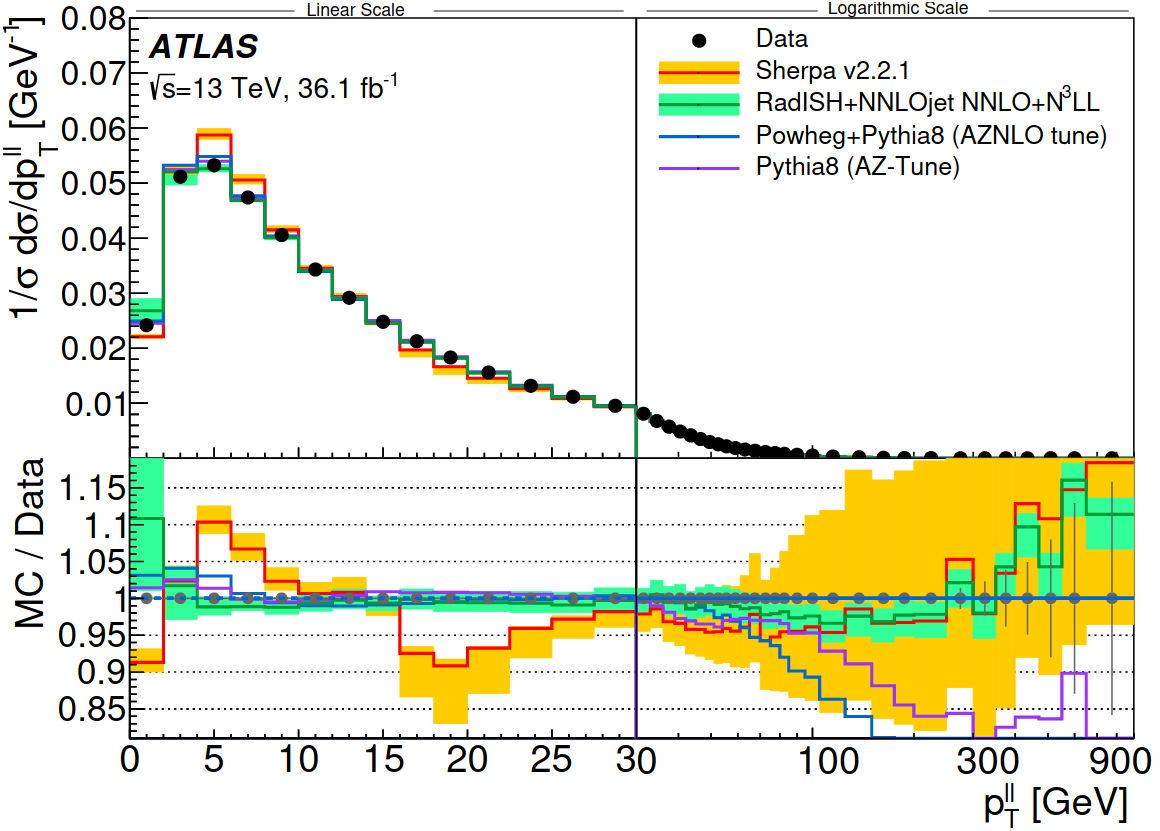
\includegraphics[width=0.6\textwidth]{figures/Fig10}
	\caption{Comparison of the Z$\pt$ modelling in Drell-Yan events made by different MC generators. As it can be seen, Sherpa does a better job describing the Z boson transverse momentum for higher Z$\pt$ values than Powheg+Pythia8. However both generators underestimate the measured value in the high-Z$\pt$ region. Taken from \cite{Aad:2019wmn}}
	\label{Fig10}
\end{figure}

Fig. \ref{Fig11}, shows the Z$\pt$ distribution for our final selected events. Looking at these plots, it is clear that $\Sherpa$ does a better for highly-boosted $\Zll$ events. The total yields for all the final states, using Sherpa samples as signal, are shown in Table \ref{Tab6}. With these figures, we calculate the C factors and the SFs reported in the second column of Table \ref{Tab7} and \ref{Tab8}. The yields for the other generator and the re-weighted samples are used to calculate the two remaining columns.

\begin{figure}[htbp]
	\centering
	\subfloat[]{\label{Fig11a}{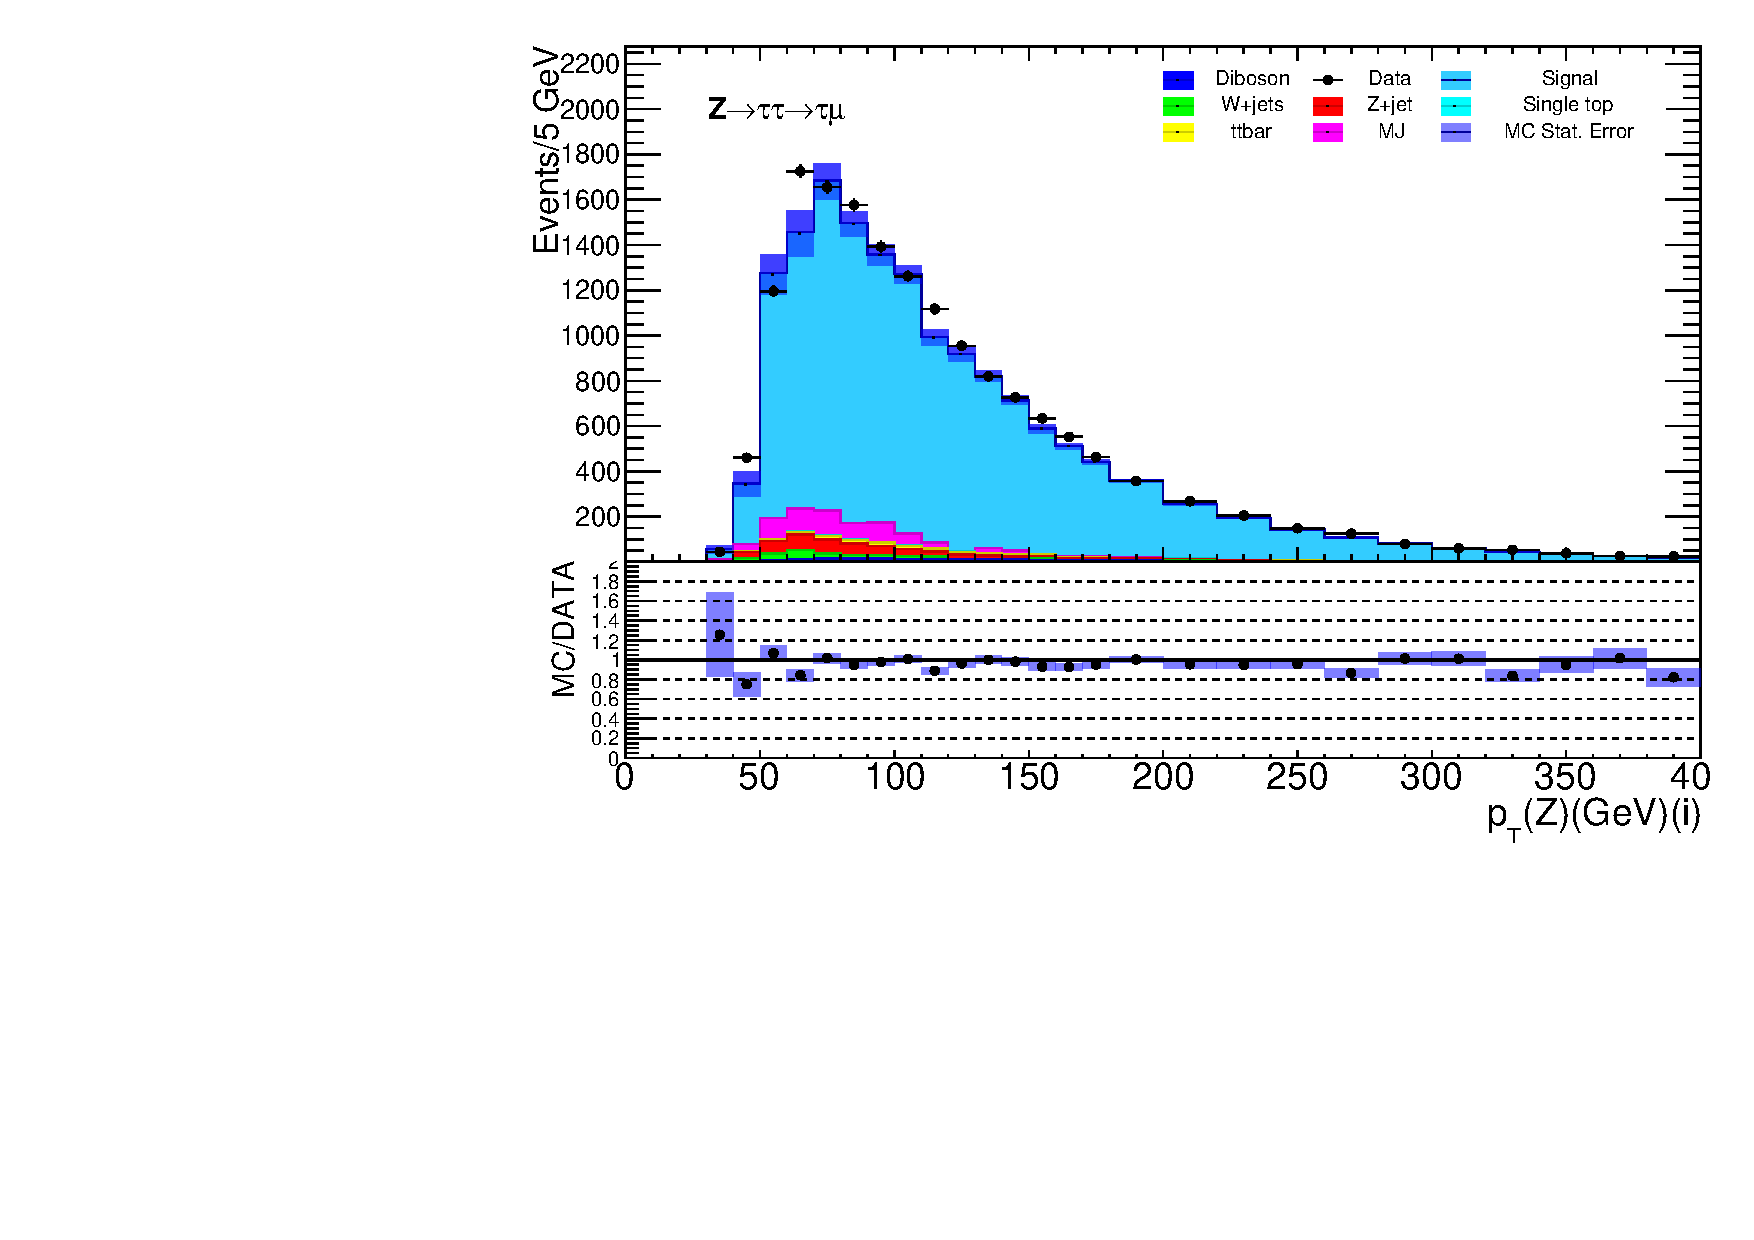
\includegraphics[width=0.50\textwidth]{figures/Fig11a}}}\hfill
	\subfloat[]{\label{Fig11b}{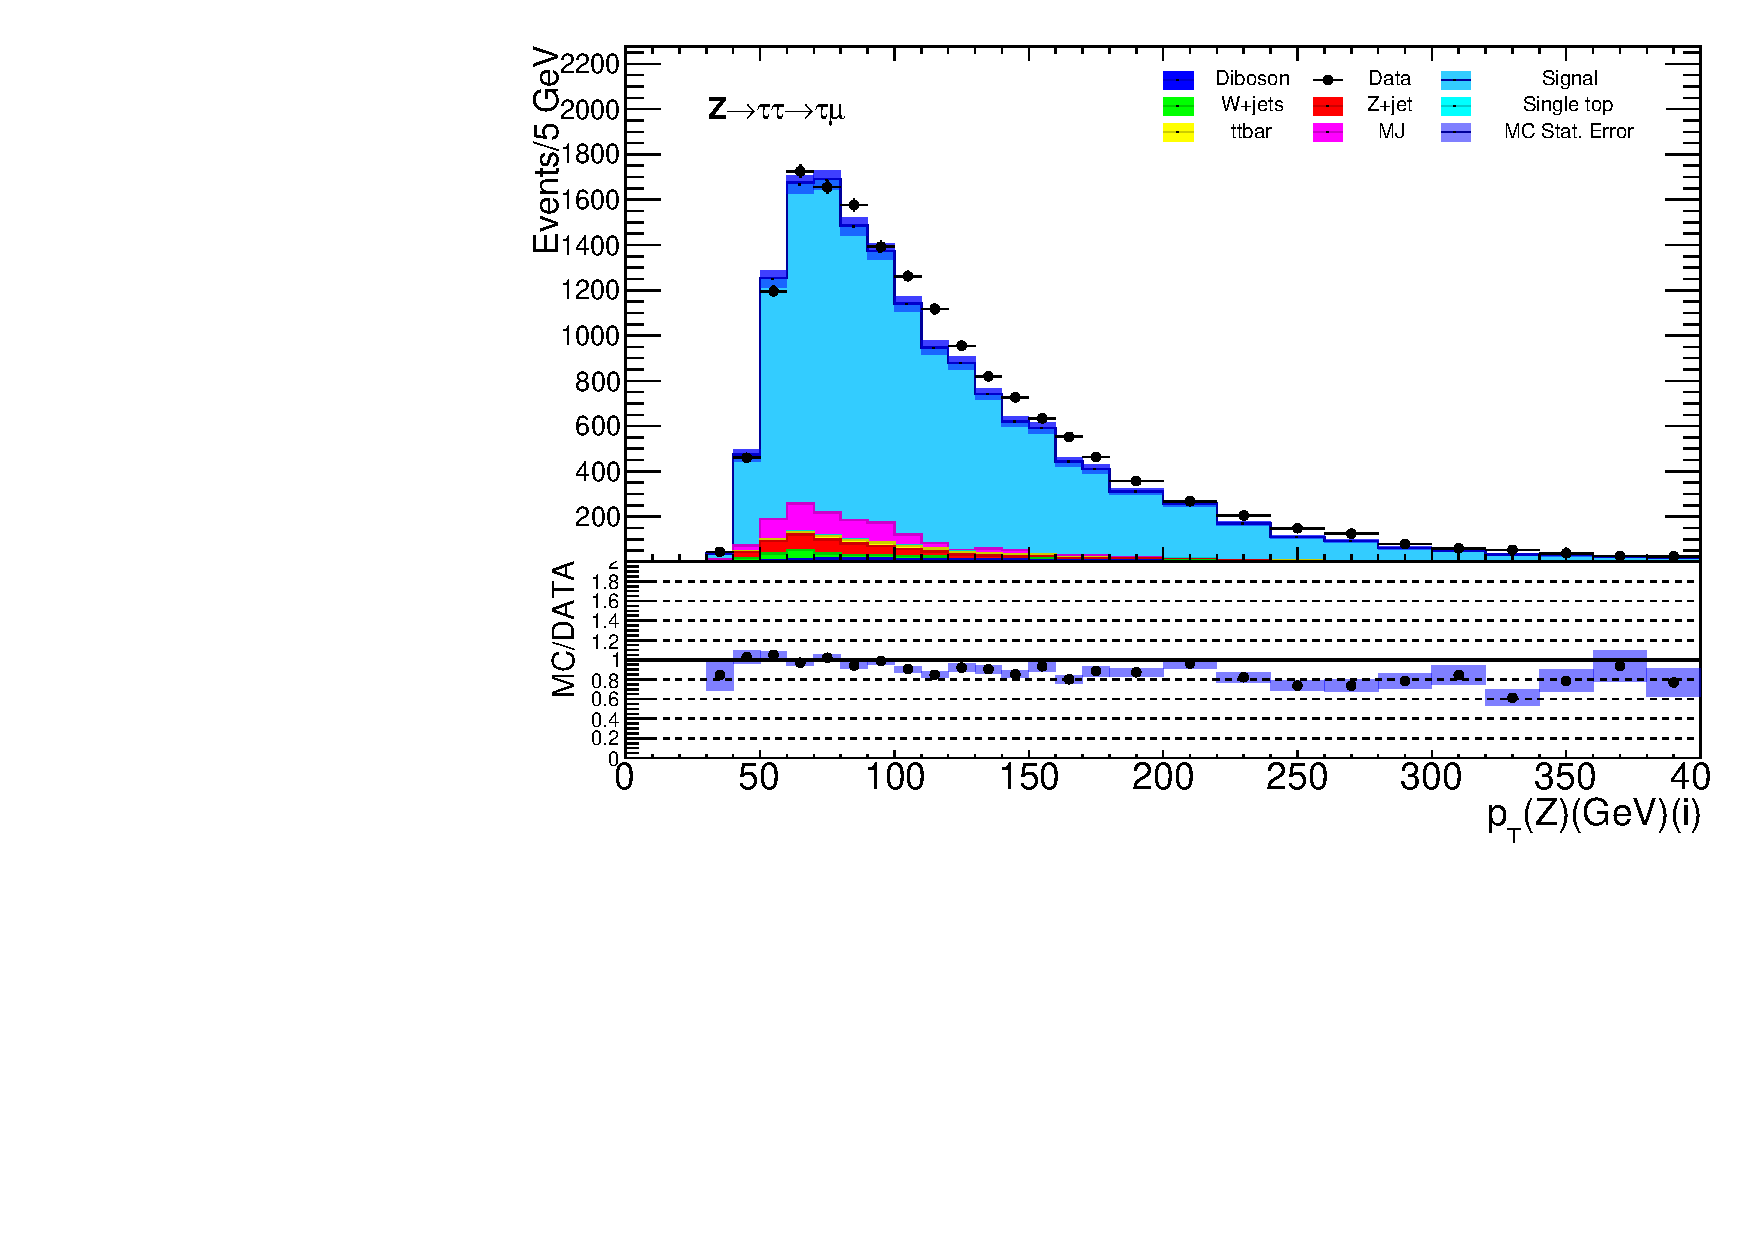
\includegraphics[width=0.50\textwidth]{figures/Fig11b}}}
	\caption{Z$\pt$ distributions for $Z\to\tauhad\mu$ events. $\Sherpa$ prediction (a) is much closer to the data. Meanwhile, $\POWPY[8]$ tends to underestimate the data increasingly as the Z$\pt$ becomes higher. }
	\label{Fig11}
\end{figure}



\begin{table}[]
	\resizebox{\textwidth}{!}{%
		\begin{tabular}{|c|c|c|c|c|c|c|}
			\hline
			\rowcolor[HTML]{FFFFFF} 
			\textbf{\textbf\{Sample/Final State\}} & \multicolumn{2}{c|}{\cellcolor[HTML]{FFFFFF}\textbf{$Z\to\tauhad \mu$}}                         & \textbf{$Z\to\mu \mu$}              & \multicolumn{2}{c|}{\cellcolor[HTML]{FFFFFF}$Z\to\tauhad e$}                                    & \textbf{$Z\to ee$} \\ \hline
			\rowcolor[HTML]{FFFFFF} 
			& \textbf{1-prong}                           & \textbf{3-prong} &                         & \textbf{1-prong} & \textbf{3-prong}                           &                                     \\ \hline
			\rowcolor[HTML]{FFFFFF} 
			\textbf{Data}                        & $11226\pm105.953$                                           & $2872\pm53.591$                   & $468309\pm684.331$                                   & $8258\pm90.874$                   & $2164\pm46.519$                                             & $349189\pm590.922$                  \\ \hline
			\rowcolor[HTML]{FFFFFF} 
			\textbf{Signal(T+F)}                 & $10141.115\pm161.843$                                       & $2974.217\pm91.924$               & $424862.08\pm1582.183$                               & $7420.613\pm132.793$              & $2119.67\pm80.01$                                           & $318455.557\pm866.114$              \\ \hline
			\rowcolor[HTML]{FFFFFF} 
			\textbf{Diboson}                     & $167.767\pm2.662$                                           & $42.741\pm1.335$                  & $7996.946\pm22.836$                                  & $130.516\pm2.394$                 & $37.799\pm1.204$                                            & $6275.035\pm17.602$                 \\ \hline
			\rowcolor[HTML]{FFFFFF} 
			\textbf{W+Jets}                      & $49.86\pm28.195$                                            & $12.663\pm13.052$                 & \multicolumn{1}{l|}{\cellcolor[HTML]{FFFFFF}$0\pm0$} & $9.914\pm10.219$                  & \multicolumn{1}{l|}{\cellcolor[HTML]{FFFFFF}$0\pm0$}        & $5.009\pm5.009$                     \\ \hline
			\rowcolor[HTML]{FFFFFF} 
			\textbf{Z+Jets}                      & $134.893\pm5.704$                                           & $0.801\pm0.535$                   & $21.198\pm6.311$                                     & $94.44\pm4.966$                   & $2.964\pm0.878$                                             & $6.706\pm3.374$                     \\ \hline
			\rowcolor[HTML]{FFFFFF} 
			\textbf{$t\bar{t}$}                  & $78.903\pm3.311$                                            & $23.564\pm1.809$                  & $321.819\pm6.853$                                    & $51.405\pm2.73$                   & $15.462\pm1.494$                                            & $246.963\pm5.964$                   \\ \hline
			\rowcolor[HTML]{FFFFFF} 
			\textbf{Single top}                  & $13.228\pm1.244$                                            & $2.584\pm0.534$                   & $53.894\pm2.687$                                     & $8.561\pm1.063$                   & \multicolumn{1}{l|}{\cellcolor[HTML]{FFFFFF}$3.35\pm0.66$}  & $38.564\pm2.274$                    \\ \hline
			\rowcolor[HTML]{FFFFFF} 
			\textbf{Multi Jet}                   & $95.615\pm34.274$                                           & $29.986\pm34.312$                 &                                                      & $73.356\pm24.249$                 & \multicolumn{1}{l|}{\cellcolor[HTML]{FFFFFF}$0\pm24.249$}   &                                     \\ \hline
			\rowcolor[HTML]{FFFFFF} 
			\textbf{RQCD}                        & \multicolumn{1}{l|}{\cellcolor[HTML]{FFFFFF}$1.155\pm0.04$} & $1.367\pm0.074$                   &                                                      & $0.957\pm0.103$                   & $1.557\pm0.215$                                             &                                     \\ \hline
			\rowcolor[HTML]{FFFFFF} 
			\textbf{Signal Truth}                & $10018.055\pm161.144$                                       & $2971.697\pm91.912$               &                                                      & $7413.946\pm132.739$              & $2119.098\pm80.009$                                         &                                     \\ \hline
			\rowcolor[HTML]{FFFFFF} 
			\textbf{Signal Fakes}                & $123.06\pm15.028$                                           & $2.521\pm1.496$                   &                                                      & $6.664\pm3.811$                   & \multicolumn{1}{l|}{\cellcolor[HTML]{FFFFFF}$0.571\pm0.42$} &                                     \\ \hline
			\multicolumn{4}{|c|}{Only Statistical uncertainty is reported.}                                                                                                                                                & \multicolumn{3}{c|}{$\Sherpa$ Used for signal samples.}                                                                               \\ \hline
		\end{tabular}%
	\caption{Yields for all the samples used in the analysis with $\Sherpa$ as signal for $\Zll$ events. The total fakes row is defined by the sum of all EW backgrounds, the MJ contribution and the fakes from the signal sample.}
	\label{Tab6}
	}
\end{table}

 \begin{table}[H]
 	\resizebox{\textwidth}{!}{%
 		\begin{tabular}{|c|c|c|c|}
 			\hline
 			\textbf{Sample (1-prong)}						  & \textbf{Sherpa}						    & PoPy-RW                       & PoPy                          \\ \hline
 			$p_T$ Range (GeV)                                 & \multicolumn{3}{c|}{$p_T>$70}                                                                           \\ \hline
 			$C(Z\to\mu\mu)$                                   & $1.083\pm0.002\pm0.004=0.004$           & $0.987\pm0.001\pm0.001=0.002$ & $1.182\pm0.002\pm0.001=0.002$ \\ \hline
 			$C(Z\to ee)$                                      & $1.076\pm0.002\pm0.003=0.003$           & $1.021\pm0.002\pm0.001=0.002$ & $1.227\pm0.002\pm0.001=0.002$ \\ \hline
 			$p_T$ Range (GeV)                                 & \multicolumn{3}{c|}{$p_T>$45}                                                                           \\ \hline
 			$C_{\text{Tight-ID}}(Z\to\tau\mu)$                & $1.054\pm0.011\pm0.017=0.021$           & $0.954\pm0.01\pm0.014=0.017$  & $1.126\pm0.012\pm0.016=0.02$  \\ \hline
 			$\text{SF}_{\text{Tight-ID}}$                     & $0.974\pm0.01\pm0.016=0.019$            & $0.967\pm0.01\pm0.014=0.017$  & $0.953\pm0.01\pm0.014=0.017$  \\ \hline
 			$C_{\text{Tight-ID}}(Z\to\tau e)$                 & $1.063\pm0.012\pm0.019=0.023$           & $0.987\pm0.011\pm0.017=0.02$  & $1.169\pm0.014\pm0.02=0.024$  \\ \hline
 			$\text{SF}_{\text{Tight-ID}}$                     & $0.988\pm0.012\pm0.018=0.022$           & $0.952\pm0.011\pm0.018=0.021$ & $0.953\pm0.011\pm0.016=0.02$  \\ \hline
 			\multicolumn{4}{|c|}{Statistical uncertainty is reported as Correlated $\pm$ Uncorrelated $=$ Total}                                                        \\ \hline
 		\end{tabular}%
 	\caption{Values obtained for the C and SFs for different generators configurations, in the case of 1-prong taus. Only the statistical uncertainty is reported. The uncorrelated uncertainties stands for the statistical fluctuations coming from the signal sample and the MJ estimation.}
 	\label{Tab7}
 	}
 \end{table}
 
 \begin{table}[H]
 	\resizebox{\textwidth}{!}{%
 		\begin{tabular}{|c|c|c|c|}
 			\hline
 			\cellcolor[HTML]{FFFFFF}\textbf{Sample (3-prong)} & \cellcolor[HTML]{FFFFFF}\textbf{Sherpa} & PoPy-RW                       & PoPy                          \\ \hline
 			$p_T$ Range (GeV)                                 & \multicolumn{3}{c|}{$p_T>$45}                                                                           \\ \hline
 			$C_{\text{Tight-ID}}(Z\to\tau\mu)$                & $0.928\pm0.019\pm0.031=0.036$           & $0.914\pm0.018\pm0.026=0.031$ & $1.072\pm0.021\pm0.03=0.037$  \\ \hline
 			$\text{SF}_{\text{Tight-ID}}$                     & $0.857\pm0.017\pm0.029=0.034$           & $0.927\pm0.018\pm0.026=0.032$ & $0.907\pm0.018\pm0.025=0.031$ \\ \hline
 			$C_{\text{Tight-ID}}(Z\to\tau e)$                 & $0.993\pm0.022\pm0.039=0.045$           & $0.875\pm0.02\pm0.029=0.035$  & $1.033\pm0.023\pm0.034=0.041$ \\ \hline
 			$\text{SF}_{\text{Tight-ID}}$                     & $0.923\pm0.02\pm0.037=0.042$            & $0.857\pm0.019\pm0.029=0.034$ & $0.841\pm0.019\pm0.028=0.034$ \\ \hline
 			\multicolumn{4}{|c|}{Statistical uncertainty is reported as Correlated $\pm$ Uncorrelated $=$ Total}                                                        \\ \hline
 		\end{tabular}%
 	\caption{Values obtained for the C and SFs for different generators configurations, in the case of 3-prong taus. Only the statistical uncertainty is reported. The uncorrelated uncertainties stands for the statistical fluctuations coming from the signal sample and the MJ estimation.}
 	\label{Tab8}
 	}
 \end{table}
 

\begin{comment}
\begin{table}[H]
\resizebox{\textwidth}{!}{%
\centering
\begin{tabular}{|c|c|c|c|} 
\hline
\rowcolor[rgb]{0.753,0.753,0.753} Sample (1-prong)                  & Sherpa                                                                 & PoPy-RW                                                                & PoPy                                                                    \\ 
\hline
\rowcolor[rgb]{0.937,0.937,0.937} $p_T$ Range (GeV)                 & \multicolumn{3}{c|}{$p_T>$70}                                                                                                                                                                                             \\ 
\hline
\rowcolor[rgb]{0.604,1,0.6} $C(Z\to\mu\mu)$                         & $1.083\pm0.002\pm0.004=0.004$ & $0.987\pm0.001\pm0.001=0.002$ & $1.182\pm0.002\pm0.001=0.002$  \\ 
\hline
\rowcolor[rgb]{0.604,1,0.6} $C(Z\to ee)$                            & $1.076\pm0.002\pm0.003=0.003$ & $1.021\pm0.002\pm0.001=0.002$ & $1.227\pm0.002\pm0.001=0.002$  \\ 
\hline
\rowcolor[rgb]{0.937,0.937,0.937} $p_T$ Range (GeV)                 & \multicolumn{3}{c|}{$p_T>$45}                                                                                                                                                                                             \\ 
\hline
\rowcolor[rgb]{0.588,1,0.984} $C_{\text{Tight-ID}}(Z\to\tau\mu)$    & $1.044\pm0.011\pm0.018=0.021$ & $0.947\pm0.01\pm0.014=0.017$  & $1.11\pm0.012\pm0.017=0.02$    \\ 
\hline
\rowcolor[rgb]{0.588,1,0.984} $\text{SF}_{\text{Tight-ID}}$                          & $0.964\pm0.01\pm0.017=0.02$   & $0.959\pm0.01\pm0.014=0.017$  & $0.939\pm0.01\pm0.014=0.017$   \\ 
\hline
\rowcolor[rgb]{0.992,0.408,0.392} $C_{\text{Tight-ID}}(Z\to\tau e)$ & $1.041\pm0.012\pm0.021=0.025$ & $0.971\pm0.011\pm0.018=0.022$ & $1.138\pm0.014\pm0.023=0.027$  \\ 
\hline
\rowcolor[rgb]{0.992,0.408,0.392} $\text{SF}_{\text{Tight-ID}}$                      & $0.968\pm0.012\pm0.02=0.023$  & $0.952\pm0.011\pm0.018=0.021$ & $0.927\pm0.011\pm0.019=0.022$  \\ 
\hline
\multicolumn{4}{|c|}{Statistical uncertainty is reported as Correlated $\pm$ Uncorrelated $=$ Total}                                                                                                                                                                                            \\
\hline
\end{tabular}
}
\end{table}


SFs 3-prong.


\begin{table}[H]
	\resizebox{\textwidth}{!}{%
		\centering
		\begin{tabular}{|c|c|c|c|} 
			\hline
			\rowcolor[rgb]{0.753,0.753,0.753} Sample (3-prong)                  & Sherpa                                                                 & PoPy-RW                                                                & PoPy                                                                    \\ 
			\hline
			\rowcolor[rgb]{0.937,0.937,0.937} $p_T$ Range (GeV)                 & \multicolumn{3}{c|}{$p_T>$45}                                                                                                                                                                                             \\ 
			\hline
			\rowcolor[rgb]{0.588,1,0.984} $C_{\text{Tight-ID}}(Z\to\tau\mu)$    & $0.924\pm0.019\pm0.038=0.042$ & $0.912\pm0.018\pm0.029=0.034$ & $1.065\pm0.021\pm0.036=0.041$  \\ 
			\hline
			\rowcolor[rgb]{0.588,1,0.984} $\text{SF}_{\text{Tight-ID}}$                          & $0.854\pm0.017\pm0.035=0.039$ & $0.925\pm0.018\pm0.029=0.034$ & $0.901\pm0.018\pm0.03=0.035$   \\ 
			\hline
			\rowcolor[rgb]{0.992,0.408,0.392} $C_{\text{Tight-ID}}(Z\to\tau e)$ & $0.993\pm0.022\pm0.052=0.057$ & $0.872\pm0.02\pm0.039=0.044$  & $1.02\pm0.023\pm0.052=0.057$   \\ 
			\hline
			\rowcolor[rgb]{0.992,0.408,0.392} $\text{SF}_{\text{Tight-ID}}$                      & $0.923\pm0.02\pm0.049=0.053$  & $0.855\pm0.019\pm0.038=0.043$ & $0.831\pm0.019\pm0.043=0.047$  \\ 
			\hline
			\multicolumn{4}{|c|}{Statistical uncertainty is reported as Correlated $\pm$ Uncorrelated $=$ Total}                                                                                                                                                                                            \\
			\hline
		\end{tabular}
	}
\end{table}

NO eBDTs

\begin{table}[H]
	\centering
	\begin{tabular}{|c|c|c|} 
		\hline
		\rowcolor[rgb]{0.753,0.753,0.753} Sample (1-prong)                  & Sherpa                                                        & PoPy-RW                                                        \\ 
		\hline
		\rowcolor[rgb]{0.937,0.937,0.937}                                   & \multicolumn{2}{c|}{No eBDT + $m(e,\tau)<80$}                                                                  \\ 
		\hline
		\rowcolor[rgb]{0.588,1,0.984} $C_{\text{Tight-ID}}(Z\to\tau e)$     & $1.002\pm0.012\pm0.024=0.027$ & $0.953\pm0.011\pm0.021=0.024$  \\ 
		\hline
		\rowcolor[rgb]{0.588,1,0.984} $\text{SF}_{\text{Tight-ID}}$                          & $0.932\pm0.011\pm0.022=0.025$ & $0.934\pm0.011\pm0.021=0.024$  \\ 
		\hline
		\multicolumn{1}{|l|}{}                                              & \multicolumn{2}{c|}{No eBDT + $m(e,\tau)<75$}                                                                  \\ 
		\hline
		\rowcolor[rgb]{0.992,0.408,0.392} $C_{\text{Tight-ID}}(Z\to\tau e)$ & $0.992\pm0.012\pm0.022=0.025$ & $0.944\pm0.012\pm0.02=0.023$   \\ 
		\hline
		\rowcolor[rgb]{0.992,0.408,0.392} $\text{SF}_{\text{Tight-ID}}$                      & $0.922\pm0.012\pm0.02=0.023$  & $0.925\pm0.012\pm0.02=0.023$   \\ 
		\hline
		\multicolumn{3}{|c|}{Statistical uncertainty is reported as Correlated $\pm$ Uncorrelated $=$ Total}                                                                                                 \\
		\hline
	\end{tabular}
\end{table}

\begin{table}[H]
	\centering
	\begin{tabular}{|c|c|c|} 
		\hline
		\rowcolor[rgb]{0.753,0.753,0.753} Sample (3-prong)                  & Sherpa                                                        & PoPy-RW                                                        \\ 
		\hline
		\rowcolor[rgb]{0.937,0.937,0.937}                                   & \multicolumn{2}{c|}{No eBDT + $m(e,\tau)<80$}                                                                                  \\ 
		\hline
		\rowcolor[rgb]{0.588,1,0.984} $C_{\text{Tight-ID}}(Z\to\tau e)$     & $0.99\pm0.022\pm0.068=0.072$  & $0.872\pm0.019\pm0.056=0.059$  \\ 
		\hline
		\rowcolor[rgb]{0.588,1,0.984} $\text{SF}_{\text{Tight-ID}}$                          & $0.921\pm0.02\pm0.064=0.067$  & $0.855\pm0.019\pm0.054=0.058$  \\ 
		\hline
		\multicolumn{1}{|l|}{}                                              & \multicolumn{2}{c|}{No eBDT + $m(e,\tau)<75$}                                                                                  \\ 
		\hline
		\rowcolor[rgb]{0.992,0.408,0.392} $C_{\text{Tight-ID}}(Z\to\tau e)$ & $0.971\pm0.022\pm0.06=0.064$  & $0.858\pm0.02\pm0.049=0.053$   \\ 
		\hline
		\rowcolor[rgb]{0.992,0.408,0.392} $\text{SF}_{\text{Tight-ID}}$                      & $0.902\pm0.021\pm0.056=0.059$ & $0.841\pm0.02\pm0.048=0.052$   \\ 
		\hline
		\multicolumn{3}{|c|}{Statistical uncertainty is reported as Correlated $\pm$ Uncorrelated $=$ Total}                                                                                                 \\
		\hline
	\end{tabular}
\end{table}

PoPy Yields

\begin{table}[H]
	\resizebox{\textwidth}{!}{%
		\begin{tabular}{|c|c|c|c|c|c|c|}
			\hline
			\rowcolor[HTML]{FFFFFF} 
			\textbf{Sample/Final State} & \multicolumn{2}{c|}{\cellcolor[HTML]{FFFFFF}\textbf{$Z\to\tauhad \mu$}} & \textbf{$Z\to\mu \mu$}        & \multicolumn{2}{c|}{\cellcolor[HTML]{FFFFFF}\textbf{$Z\to\tauhad e$}} & \textbf{$Z\to ee$}            \\ \hline
			\rowcolor[HTML]{FFFFFF} 
			& \textbf{1-prong}                   & \textbf{3-prong}                   & \textbf{}                     & \textbf{1-prong}                  & \textbf{3-prong}                  &                               \\ \hline
			\rowcolor[HTML]{FFFFFF} 
			\textbf{Data}               & $11226\pm105.953$                  & $2872\pm53.591$                    & $468309\pm684.331$            & $8258\pm90.874$                   & $2164\pm46.519$                   & $349189\pm590.922$            \\ \hline
			\rowcolor[HTML]{FFFFFF} 
			\textbf{Signal(T+F)}        & $9463.807\pm132.039$               & $2592.277\pm68.734$                & $389244.279\pm320.997$        & $6735.205\pm112.939$              & $2016.842\pm61.737$               & $279172.354\pm258.624$        \\ \hline
			\rowcolor[HTML]{FFFFFF} 
			\textbf{Diboson}            & $167.767\pm2.662$                  & $42.741\pm1.335$                   & $7996.946\pm22.836$           & $130.516\pm2.394$                 & $37.799\pm1.204$                  & $6275.035\pm17.602$           \\ \hline
			\rowcolor[HTML]{FFFFFF} 
			\textbf{W+Jets}             & $49.86\pm28.195$                   & $12.663\pm13.052$                  & $0\pm0$                       & $9.914\pm10.219$                  & $0\pm0$                           & $5.009\pm5.009$               \\ \hline
			\rowcolor[HTML]{FFFFFF} 
			\textbf{Z+Jets}             & $134.893\pm5.704$                  & $0.801\pm0.535$                    & $21.198\pm6.311$              & $94.44\pm4.966$                   & $2.964\pm0.878$                   & $6.706\pm3.374$               \\ \hline
			\rowcolor[HTML]{FFFFFF} 
			\textbf{$t\bar{t}$}         & $78.903\pm3.311$                   & $23.564\pm1.809$                   & $321.819\pm6.853$             & $51.405\pm2.73$                   & $15.462\pm1.494$                  & $246.963\pm5.964$             \\ \hline
			\rowcolor[HTML]{FFFFFF} 
			\textbf{Single top}         & $13.228\pm1.244$                   & $2.584\pm0.534$                    & $53.894\pm2.687$              & $8.561\pm1.063$                   & $3.35\pm0.66$                     & $38.564\pm2.274$              \\ \hline
			\rowcolor[HTML]{FFFFFF} 
			\textbf{Multi Jet}          & $290.142\pm55.655$                 & $29.311\pm55.823$                  &                               & $297.579\pm83.711$                & $46.753\pm84.392$                 &                               \\ \hline
			\rowcolor[HTML]{FFFFFF} 
			\textbf{RQCD}               & $2.557\pm0.154$                    & $3.325\pm0.49$                     &                               & $3.354\pm0.26$                    & $3.626\pm0.83$                    &                               \\ \hline
			\rowcolor[HTML]{FFFFFF} 
			\textbf{Signal Truth}       & $9375.435\pm131.447$               & $2592.277\pm68.734$                &                               & $6728.238\pm112.885$              & $2016.842\pm61.737$               &                               \\ \hline
			\rowcolor[HTML]{FFFFFF} 
			\textbf{Signal Fakes}       & $88.372\pm12.482$                  & $0\pm0$                            &                               & $6.967\pm3.503$                   & $0\pm0$                           &                               \\ \hline
			\rowcolor[HTML]{FFFFFF} 
			\textbf{C Factor}           & $1.11\pm0.012\pm0.017=0.02$        & $1.065\pm0.021\pm0.036=0.041$      & $1.182\pm0.002\pm0.001=0.002$ & $1.138\pm0.014\pm0.023=0.027$     & $1.02\pm0.023\pm0.052=0.057$      & $1.227\pm0.002\pm0.001=0.002$ \\ \hline
			\rowcolor[HTML]{FFFFFF} 
			\textbf{SF Factor}          & $0.939\pm0.01\pm0.014=0.017$       & $0.901\pm0.018\pm0.03=0.035$       &                               & $0.927\pm0.011\pm0.019=0.022$     & $0.831\pm0.019\pm0.043=0.047$     &                               \\ \hline
			\multicolumn{4}{|c|}{Statistical uncertainty is reported as Correlated $\pm$ Uncorrelated $=$ Total}                                  & \multicolumn{3}{c|}{PowHeg+Pythia8 Used for signal samples.}                                          \\ \hline
		\end{tabular}%
		\caption{Systematic uncertainties used in this study. At the time of writing this report we have not directly estimated all of our systematic uncertainties. However, we expect that some of them will get reduced by the double ratio method.}
		\label{Tab4}
	}
\end{table}

Low-$\pt$ study

\begin{table}[H]
	\resizebox{\textwidth}{!}{%
		\begin{tabular}{|c|c|c|c|}
			\hline
			\rowcolor[HTML]{C0C0C0} 
			\textbf{Sample (1-prong)}                         & \textbf{Sherpa}               & \textbf{PoPy-RW}              & \textbf{PoPy}                 \\ \hline
			\rowcolor[HTML]{C0C0C0} 
			\textbf{$p_T$ Range}                              & \multicolumn{3}{c|}{\cellcolor[HTML]{C0C0C0}\textbf{$p_T<45$ GeV\}}}                          \\ \hline
			\rowcolor[HTML]{67FD9A} 
			\textbf{$C(Z    \to\mu\mu)$}                      & $1.076\pm0.001\pm0.003=0.003$ & $0.996\pm0.001\pm0.001=0.001$ & $1.109\pm0.001\pm0.001=0.002$ \\ \hline
			\rowcolor[HTML]{67FD9A} 
			\textbf{$C(Z    \to ee)$}                         & $1.073\pm0.002\pm0.004=0.004$ & $1.017\pm0.002\pm0.001=0.002$ & $1.136\pm0.002\pm0.001=0.002$ \\ \hline
			\rowcolor[HTML]{34CDF9} 
			\textbf{$C_{\text{Tight-ID}}(Z\to\tau\mu)$}       & $1.002\pm0.013\pm0.023=0.027$ & $0.926\pm0.012\pm0.014=0.019$ & $1.016\pm0.014\pm0.017=0.021$ \\ \hline
			\rowcolor[HTML]{34CDF9} 
			\textbf{$\text{SF}_{\text{Tight-ID}}$} & $0.931\pm0.012\pm0.022=0.025$ & $0.93\pm0.012\pm0.014=0.019$  & $0.916\pm0.012\pm0.015=0.019$ \\ \hline
			\rowcolor[HTML]{FD6864} 
			\textbf{$C_{\text{Tight-ID}}(Z\to\tau e)$}        & $0.993\pm0.013\pm0.032=0.035$ & $0.895\pm0.012\pm0.02=0.023$  & $0.971\pm0.013\pm0.024=0.028$ \\ \hline
			\rowcolor[HTML]{FD6864} 
			\textbf{$\text{SF}_{\text{Tight-ID}}$} & $0.925\pm0.013\pm0.03=0.033$  & $0.88\pm0.012\pm0.02=0.023$   & $0.855\pm0.012\pm0.021=0.024$ \\ \hline
		\end{tabular}%
	}
\end{table}

\begin{table}[H]
	\resizebox{\textwidth}{!}{%
		\begin{tabular}{|c|c|c|c|}
			\hline
			\rowcolor[HTML]{C0C0C0} 
			\textbf{Sample (3-prong)}                         & \textbf{Sherpa}               & \textbf{PoPy-RW}              & \textbf{PoPy}                 \\ \hline
			\rowcolor[HTML]{C0C0C0} 
			\textbf{$p_T$ Range}                              & \multicolumn{3}{c|}{\cellcolor[HTML]{C0C0C0}\textbf{$p_T<45$ GeV\}}}                          \\ \hline
			\rowcolor[HTML]{34CDF9} 
			\textbf{$C_{\text{Tight-ID}}(Z\to\tau\mu)$}       & $0.976\pm0.016\pm0.075=0.077$ & $0.886\pm0.015\pm0.052=0.054$ & $0.96\pm0.017\pm0.062=0.065$  \\ \hline
			\rowcolor[HTML]{34CDF9} 
			\textbf{$\text{SF}_{\text{Tight-ID}}$} & $0.908\pm0.015\pm0.07=0.072$  & $0.89\pm0.016\pm0.052=0.054$  & $0.866\pm0.015\pm0.056=0.058$ \\ \hline
			\rowcolor[HTML]{FD6864} 
			\textbf{$C_{\text{Tight-ID}}(Z\to\tau e)$}        & $0.917\pm0.019\pm0.108=0.11$  & $0.887\pm0.018\pm0.08=0.082$  & $0.951\pm0.02\pm0.098=0.1$    \\ \hline
			\rowcolor[HTML]{FD6864} 
			\textbf{$\text{SF}_{\text{Tight-ID}}$} & $0.854\pm0.018\pm0.101=0.102$ & $0.872\pm0.017\pm0.079=0.081$ & $0.837\pm0.017\pm0.086=0.088$ \\ \hline
		\end{tabular}%
	}
\end{table}

Anti-ID RNN Control Region Def

\begin{table}[H]
	\resizebox{\textwidth}{!}{%
		\begin{tabular}{|c|c|c|c|}
			\hline
			\textbf{Sample (1-prong)}						  & \textbf{Sherpa}						    & PoPy-RW                       & PoPy                          \\ \hline
			$p_T$ Range (GeV)                                 & \multicolumn{3}{c|}{$p_T>$70}                                                                           \\ \hline
			$C(Z\to\mu\mu)$                                   & $1.083\pm0.002\pm0.004=0.004$           & $0.987\pm0.001\pm0.001=0.002$ & $1.182\pm0.002\pm0.001=0.002$ \\ \hline
			$C(Z\to ee)$                                      & $1.076\pm0.002\pm0.003=0.003$           & $1.021\pm0.002\pm0.001=0.002$ & $1.227\pm0.002\pm0.001=0.002$ \\ \hline
			$p_T$ Range (GeV)                                 & \multicolumn{3}{c|}{$p_T>$45}                                                                           \\ \hline
			$C_{\text{Tight-ID}}(Z\to\tau\mu)$                & $1.054\pm0.011\pm0.017=0.021$           & $0.954\pm0.01\pm0.014=0.017$  & $1.126\pm0.012\pm0.016=0.02$  \\ \hline
			$\text{SF}_{\text{Tight-ID}}$                     & $0.974\pm0.01\pm0.016=0.019$            & $0.967\pm0.01\pm0.014=0.017$  & $0.953\pm0.01\pm0.014=0.017$  \\ \hline
			$C_{\text{Tight-ID}}(Z\to\tau e)$                 & $1.063\pm0.012\pm0.019=0.023$           & $0.987\pm0.011\pm0.017=0.02$  & $1.169\pm0.014\pm0.02=0.024$  \\ \hline
			$\text{SF}_{\text{Tight-ID}}$                     & $0.988\pm0.012\pm0.018=0.022$           & $0.952\pm0.011\pm0.018=0.021$ & $0.953\pm0.011\pm0.016=0.02$  \\ \hline
			\multicolumn{4}{|c|}{Statistical uncertainty is reported as Correlated $\pm$ Uncorrelated $=$ Total}                                                        \\ \hline
		\end{tabular}%
	}
\end{table}

\begin{table}[H]
	\resizebox{\textwidth}{!}{%
		\begin{tabular}{|c|c|c|c|}
			\hline
			\cellcolor[HTML]{FFFFFF}\textbf{Sample (3-prong)} & \cellcolor[HTML]{FFFFFF}\textbf{Sherpa} & PoPy-RW                       & PoPy                          \\ \hline
			$p_T$ Range (GeV)                                 & \multicolumn{3}{c|}{$p_T>$45}                                                                           \\ \hline
			$C_{\text{Tight-ID}}(Z\to\tau\mu)$                & $0.928\pm0.019\pm0.031=0.036$           & $0.914\pm0.018\pm0.026=0.031$ & $1.072\pm0.021\pm0.03=0.037$  \\ \hline
			$\text{SF}_{\text{Tight-ID}}$                     & $0.857\pm0.017\pm0.029=0.034$           & $0.927\pm0.018\pm0.026=0.032$ & $0.907\pm0.018\pm0.025=0.031$ \\ \hline
			$C_{\text{Tight-ID}}(Z\to\tau e)$                 & $0.993\pm0.022\pm0.039=0.045$           & $0.875\pm0.02\pm0.029=0.035$  & $1.033\pm0.023\pm0.034=0.041$ \\ \hline
			$\text{SF}_{\text{Tight-ID}}$                     & $0.923\pm0.02\pm0.037=0.042$            & $0.857\pm0.019\pm0.029=0.034$ & $0.841\pm0.019\pm0.028=0.034$ \\ \hline
			\multicolumn{4}{|c|}{Statistical uncertainty is reported as Correlated $\pm$ Uncorrelated $=$ Total}                                                        \\ \hline
		\end{tabular}%
	}
\end{table}
\end{comment}